\subsection{Literaturrecherche}
Nach \cite{vom_Brooke_2009} steht im dritten Schritt des Vorgehens (vgl. \ref{Fig:vomBrocke} das Finden der Literatur an, indem Journal- und Wissensdatenbanken mittels Stichworten durchsucht werden, worauf folgend optional eine Vorwärts- und Rückwärtssuche durchgeführt werden kann.
Gesucht wurde im Juni und Juli 2022 auf Englisch in folgenden Datenbanken: IEEE, ACM \footnote{https://dl.acm.org/}, Computer Science Bibliography \footnote{http://dblp.uni-trier.de/} sowie Google Scholar \footnote{https://scholar.google.com/}. zusätzlich wurde noch die reguläre Suchmaschine \textit{Google} genutzt, da sich die Handreichung schließlich an Prakitker richten soll und somit auch Ansätze aus der Praxis, z.B. von Beratungshäusern oder großen Software-Firmen nicht ausgeschlossen werden sollten \todo{Das muss ich noch machen}.

Um die Anzahl der zu betrachtenden Publikationen und Beiträge überschaubar zu halten, wurden in wissenschaftlichen Datenbanken für RQ 1 die ersten 200 betrachtet. Da für die erste Forschungsfrage bereits viele wissenschaftlichen Quellen (296) gefunden wurde, die bereits auf Tranpsarenz bei konkreten ML-Methoden eingingen, wurde sich entschieden in Bezug auf RQ2 lediglich eine ergänzende Literaturrecherche durchzuführen, um zum einen keine relevanten transparenzschaffenden Methoden zu übersehen, jedoch zum anderen auf die Dokumentation aller gefundenen Literatur zu verzichten, um den zeitlichen und inhaltlichen Rahmen nicht zu sprengen.
- Google für transparenz in Machine Learning um keine in der Praxis relevanten Sachen zu verpassen (hierfür ersten 50 Ergebnisse von Websites)
- für RQ2: lesen des Titels und Abstract und dann Aufnahme in den Literaturpool (hierfür wurden die ersten 50 Ergebnisse von Google Scholar je Suchtherm  betrachtet)
- für die ergänzende Literaturrecherche wurden Duplikate nicht mit in die Dokumentation aufgenommen, sondern nur das was inhaltlich neu war


\begin{figure}
    \centering
    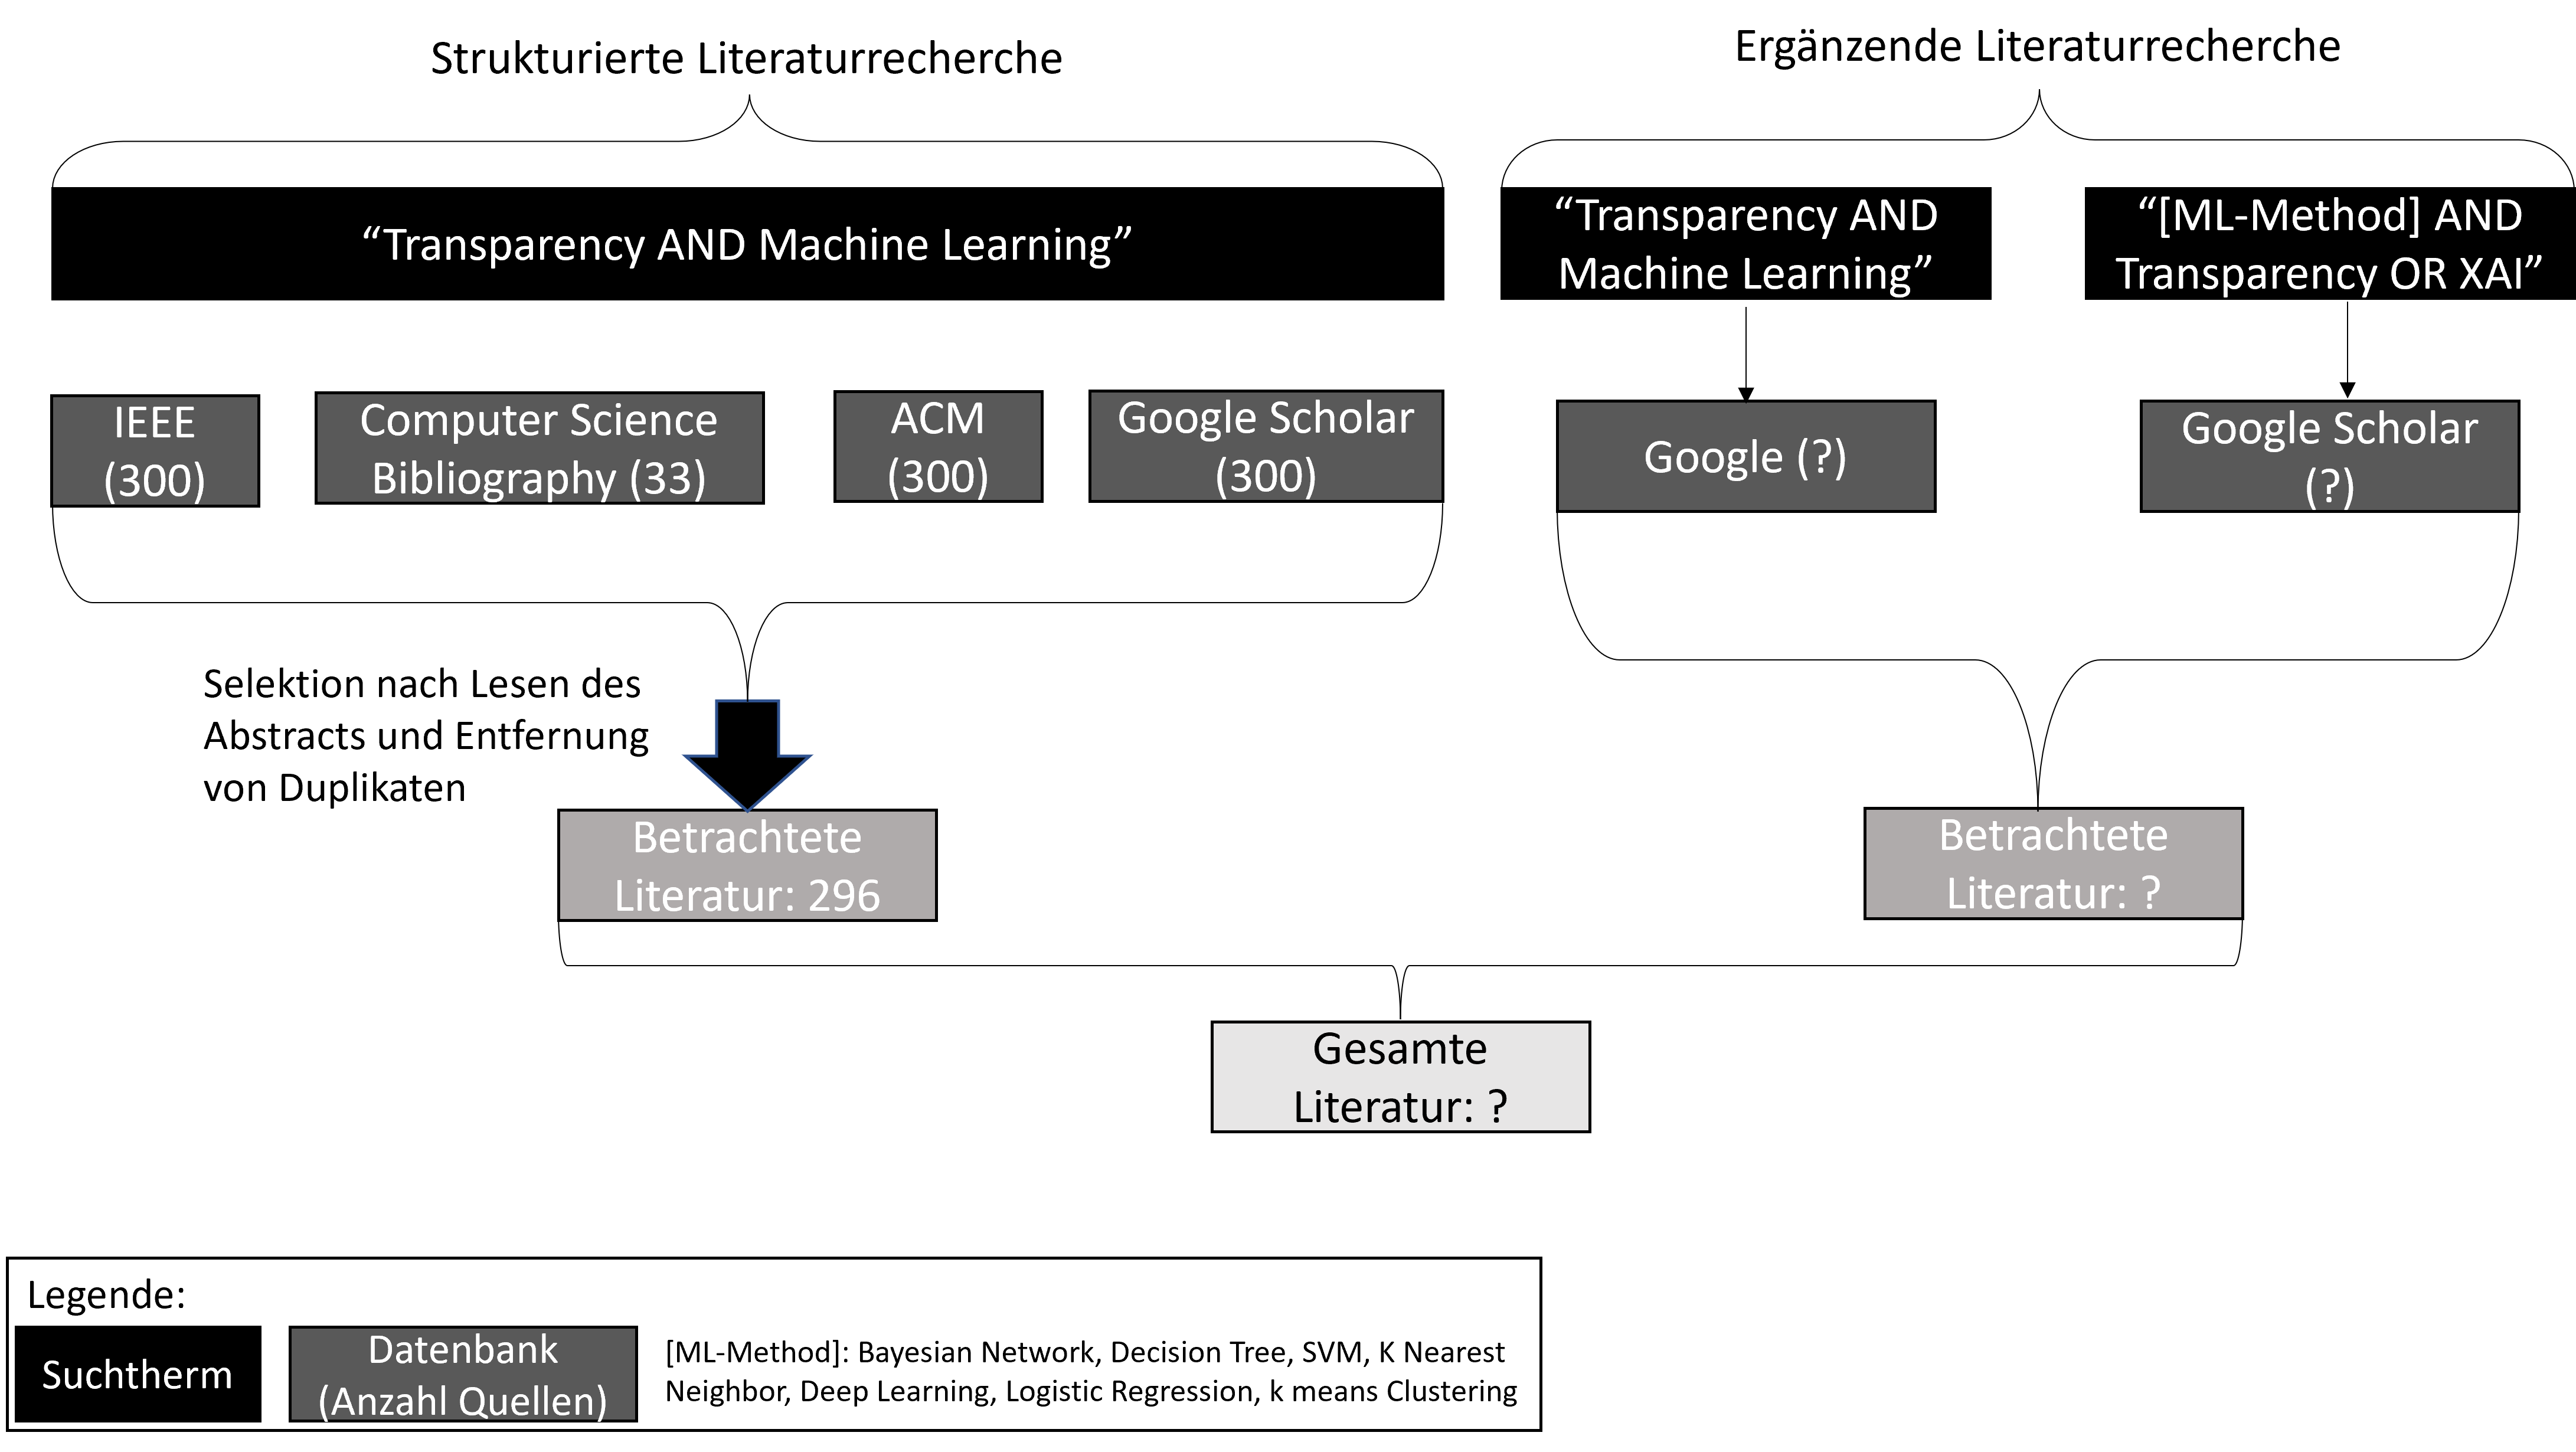
\includegraphics[scale=0.45]{pic/MA-Bilder/Literaturrecherche.png}
    \caption{Vorgehen bei der Literatursuche, eigene Darstellung}
    \label{Fig:Literatursuche}
\end{figure}

Eine Überblick über die verschiedenen Datenbanken, Suchterme und -ergebnisse findet sich im Anhang.